% Tiga Garis di Atas Histogram: Mean, Median, Modus dengan TikZ
% Dokumen LaTeX utuh, siap dikompilasi (butuh paket tikz).
% Data: 32 nilai ulangan harian Matematika kelas 8C, dikelompokkan.
% 40-49: 2 | 50-59: 4 | 60-69: 7 | 70-79: 9 | 80-89: 7 | 90-100: 3
% Rata-rata = 72,0 | Median = 72,8 | Modus = 74,5
\documentclass{article}
\usepackage{tikz}

\begin{document}

\section*{Histogram + tiga ukuran pemusatan}

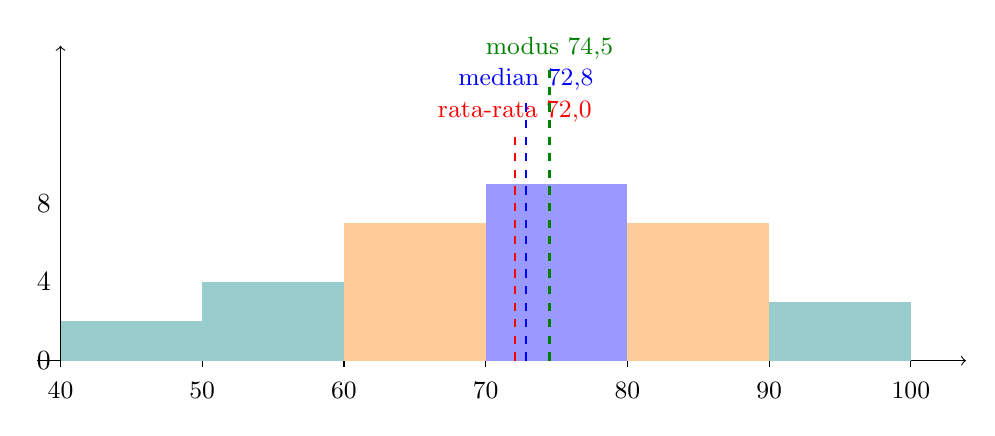
\begin{tikzpicture}
  % skala sumbu x: 0,18 cm untuk tiap 1 nilai (nilai 40 -> x=0 ; nilai 100 -> x=10,8)
  % skala sumbu y: 1 cm = 4 anak, sumbu frekuensi mulai dari NOL
  \draw[->] (-0.3,0) -- (11.5,0);
  \draw[->] (0,0) -- (0,4);
  % tanda nilai pada sumbu x
  \foreach \v in {40,50,60,70,80,90,100}
    { \pgfmathsetmacro{\x}{(\v-40)*0.18}
      \draw (\x,0) -- (\x,-0.08);
      \node[below, font=\small] at (\x,-0.15) {\v}; }
  % skala frekuensi
  \foreach \y/\label in {0/0, 1/4, 2/8}
    \node[left] at (0,\y) {\label};
  % histogram: interval 40-50 digambar dari x=0 s.d. 1,8 dst.; tinggi = f/4
  \fill[teal!40]   (0,0) rectangle (1.8,0.5);    % 40-49: 2
  \fill[teal!40]   (1.8,0) rectangle (3.6,1);    % 50-59: 4
  \fill[orange!40] (3.6,0) rectangle (5.4,1.75); % 60-69: 7
  \fill[blue!40]   (5.4,0) rectangle (7.2,2.25); % 70-79: 9
  \fill[orange!40] (7.2,0) rectangle (9,1.75);   % 80-89: 7
  \fill[teal!40]   (9,0) rectangle (10.8,0.75);  % 90-100: 3
  % tiga garis tegak (putus-putus); label disusun bertingkat agar tidak bertumpuk
  \draw[red, thick, dashed] (5.77,0) -- (5.77,2.9)
    node[above, font=\small, red] {rata-rata 72,0};
  \draw[blue, thick, dashed] (5.91,0) -- (5.91,3.3)
    node[above, font=\small, blue] {median 72,8};
  \draw[green!50!black, thick, dashed] (6.21,0) -- (6.21,3.7)
    node[above, font=\small, green!50!black] {modus 74,5};
\end{tikzpicture}

\end{document}
